\documentclass[tikz,border=4pt]{standalone}
\usepackage{amsmath}
\begin{document}
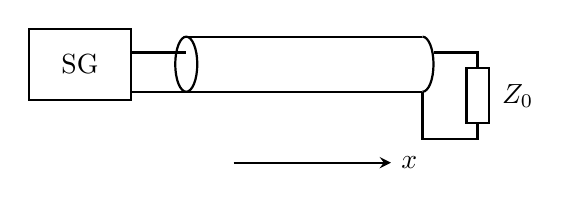
\begin{tikzpicture}[>=stealth, thick, scale=1.0]
  % Signal generator
  \draw[thick] (-1.6, -0.45) rectangle (-0.3, 0.45);
  \node at (-0.95, 0) {SG};

  % Coaxial cable body
  \draw[thick] (0.4, 0.35) -- (3.4, 0.35);
  \draw[thick] (0.4, -0.35) -- (3.4, -0.35);
  \draw[thick] (0.4, 0) ellipse (0.14 and 0.35);
  \draw[thick] (3.4, 0.35) arc (90:-90:0.14 and 0.35);

  % Connections left
  \draw[thick] (-0.3, 0.15) -- (0.4, 0.15);
  \draw[thick] (-0.3, -0.35) -- (0.4, -0.35);

  % Termination resistor Z_0 on right
  \draw[thick] (3.54, 0.15) -- (4.1, 0.15) -- (4.1, -0.05);
  \draw[thick] (3.96, -0.05) rectangle (4.24, -0.75);
  \node[right] at (4.28, -0.4) {$Z_0$};
  \draw[thick] (4.1, -0.75) -- (4.1, -0.95) -- (3.4, -0.95) -- (3.4, -0.35);

  % x axis
  \draw[->] (1.0, -1.25) -- (3.0, -1.25) node[right] {$x$};
\end{tikzpicture}
\end{document}
